%%%%%%%%%%%%%%%%%%%%%%%%%%%%%%%%%%%%%%%%%%%%%%%%%%%%%%%%%%%%%%%%%%%%%%
%Introdução
%○ Contextualização do Problema
%   ■ Descrição
%   ■ Justificativa
%○ Normalização
%○ Projeto Lógico/Relacional
%○ Projeto Conceitual
%   ■ Modelo/Diagrama ER
%○ Projeto Físico
%   ■ DDLs (CREATEs TABLE…)
%       ● Modelo/Diagrama ERD
%   ■ Polulação dos Dados
%   ■ DMLs (SELECTs…Consultas/Views)
% ○ Lições Aprendidas
% ○ Referências


%
%%%%%%%%%%%%%%%%%%%%%%%%%%%%%%%%%%%%%%%%%%%%%%%%%%%%%%%%%%%%%%%%%%%%%%

\documentclass[12pt]{article}

\usepackage{sbc-template}

\usepackage{graphicx,url}

%\usepackage[brazil]{babel}   
\usepackage[utf8]{inputenc}  

     
\sloppy

\title{Trabalho de Banco de Dados - Grupo 19 - Censo das INSTITUIÇÕES - Educação Superior - 2022}

\author{Tadeu Brasil de Souza\inst{1}, Joao Victor Rodriguez\inst{1} }


\address{
  Banco de Dados\\
  Universidade Federal do Pampa (UNIPAMPA) -- Alegrete, RS -- Brazil
  \email{\{tadeusouza.aluno@unipampa.edu.br, joaorodriguez.aluno@unipampa.edu.br}
}

\begin{document} 

\maketitle

\begin{abstract}
 Exploration and Application of Relational Database Modeling"

This project aims to delve into the extensive realm of relational database modeling, exploring techniques and methods for analyzing, designing, and manipulating models, schemas, and information. Building upon the concepts learned in the course, the scope focuses on the practical development of a comprehensive database project.

The challenge involves working in pairs to develop a database project encompassing a chosen system, utilizing a validated public database approved by the instructor. The process entails creating conceptual, logical-relational, and physical models, incorporating normalization and generating SQL instructions (DDL and DML).

Operationalization requires thorough research and careful selection of a relevant public database that aligns with the interests of the pair. Validation of this choice is crucial and will be done jointly with the instructor. Participants can explore specific portals to find suitable databases, ensuring the quality and relevance of the project
\end{abstract}
     
\begin{resumo} 
  Exploração e Aplicação de Modelagem de Bancos de Dados Relacionais"

Este trabalho se propõe a mergulhar no vasto universo da modelagem de bancos de dados relacionais, explorando técnicas e métodos para análise, projeção e manipulação de modelos, esquemas e informações. Com base nos conceitos adquiridos na disciplina, o escopo se concentra na elaboração prática de um projeto de banco de dados completo.

O desafio consiste em desenvolver, em duplas, o projeto de um banco de dados abarcando um sistema à escolha, utilizando uma base de dados pública validada pelo professor. O processo contempla a criação dos modelos conceitual, lógico-relacional e físico, incorporando a normalização e a geração de instruções SQL (DDL e DML).

A operacionalização demanda pesquisa e seleção criteriosa da base de dados pública mais relevante para os interesses da dupla. A validação dessa escolha é essencial e será realizada em conjunto com o professor. Os participantes podem explorar portais específicos para encontrar bases de dados adequadas, garantindo assim a qualidade e pertinência do projeto.
\end{resumo}

\section{Glossario}

\begin{enumerate}
 Introdução
    \item Contextualização do Problema
    \item Descrição
    \item Justificativa
    \item Normalização
    \item Projeto Lógico/Relacional
    \item Projeto Conceitual
    \item Modelo/Diagrama ER
    \item Projeto Físico
    \item DDLs (CREATEs TABLE…)
    \item Modelo/Diagrama ERD
    \item Polulação dos Dados
    \item DMLs (SELECTs…Consultas/Views)
\end{enumerate}


\section{Introdução}

Explorando a Modelagem de Banco de Dados Relacionais: Um Estudo de Caso do Censo das Instituições de Educação Superior - 2022"

No cenário em constante evolução da gestão de dados, compreender as técnicas de modelagem de banco de dados relacionais permanece fundamental. Este projeto embarca em uma jornada pelas complexidades do design e manipulação de bancos de dados, focando na análise abrangente e aplicação dessas metodologias.

O ponto central deste empreendimento é a minuciosa exploração do Censo das Instituições de Educação Superior referente ao ano de 2022. Ao navegar por este rico conjunto de dados, nosso objetivo é dissecar, analisar e, por fim, modelar a intrincada teia de informações relacionadas às instituições de ensino. Este projeto abrangerá a aplicação de técnicas de modelagem conceitual, lógico-relacional e física para encapsular as diversas dimensões deste conjunto de dados.

Por meio de esforços colaborativos e pesquisa orientada, pretendemos revelar as complexidades inerentes a este conjunto de dados e ilustrar o poder e relevância do uso de técnicas apropriadas de modelagem de bancos de dados. Esta introdução prepara o terreno para uma jornada abrangente pelos domínios da modelagem de dados, aproveitando um conjunto de dados específico para elucidar a aplicação prática desses princípios em um contexto do mundo real.


\section{Contextualização do Problema} \label{sec:firstpage}
O registro detalhado e organizado dos dados das instituições de ensino superior em bancos de dados desempenha um papel crucial em diversas esferas, oferecendo uma base sólida para análises, tomadas de decisão e aprimoramento contínuo do sistema educacional. Essa catalogação precisa e estruturada se revela essencial por várias razões, como por exemplo:

\begin{itemize}
    \item Avaliação de Qualidade Educacional: O acompanhamento de indicadores-chave, como taxas de graduação, desempenho acadêmico e recursos disponíveis, permite uma avaliação precisa da qualidade do ensino em diferentes instituições. Isso possibilita identificar áreas de excelência e necessidades de melhoria.

    \item Planejamento Estratégico: Com dados confiáveis sobre a infraestrutura, programas oferecidos, corpo docente e estudantil, é viável realizar um planejamento estratégico mais eficaz para atender às demandas educacionais. Isso inclui decidir sobre novos cursos, investimentos em recursos ou ampliação de instalações.

    \item Equidade e Acesso: O registro adequado de dados permite monitorar a distribuição geográfica das instituições e identificar desigualdades no acesso à educação superior. Essas informações são fundamentais para políticas que buscam promover a equidade no acesso à educação.

    \item Análises e Pesquisas: Bancos de dados bem-estruturados permitem análises aprofundadas sobre tendências educacionais, padrões demográficos dos estudantes, eficácia de programas acadêmicos e outras pesquisas essenciais para o avanço do campo educacional.

    \item Transparência e Prestação de Contas: Ter dados disponíveis e acessíveis promove transparência nas atividades das instituições, permitindo a prestação de contas tanto para órgãos reguladores quanto para a comunidade acadêmica e o público em geral.
\end{itemize}
Em resumo, a centralização e organização dos dados das instituições de ensino superior em bancos de dados fornecem uma base sólida para análises críticas, decisões informadas e políticas educacionais eficazes, contribuindo para o aprimoramento contínuo do sistema educacional em direção a um futuro mais inclusivo e qualitativo.



\section{Normalização}

A forma não normalizada, da forma que foi encontrado o problema:

\begin{figure}[h]
\centering
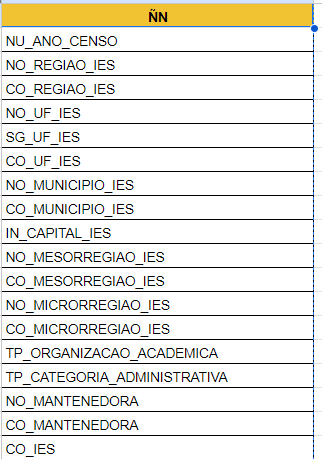
\includegraphics[width=.3\textwidth]{Nao nominal 1.PNG}
\caption{.}

\centering
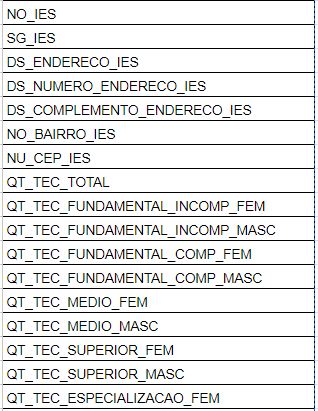
\includegraphics[width=.3\textwidth]{Nao nominal 2.PNG}
\caption{.}

\centering
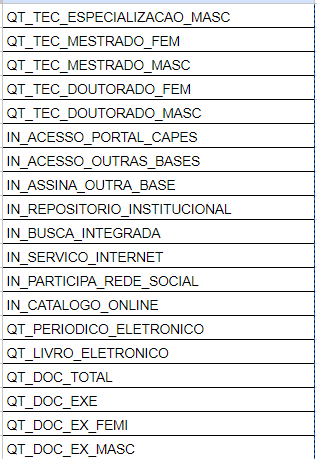
\includegraphics[width=.3\textwidth]{Nao nominal 3.PNG}
\caption{.}

\centering
\includegraphics[width=.3\textwidth]{Não nominal 4.PNG}
\caption{.}

\centering
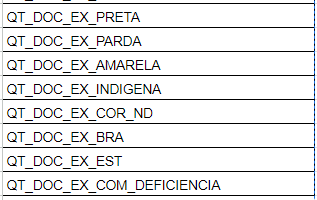
\includegraphics[width=.3\textwidth]{Nao nominal 5.PNG}
\caption{.}
\end{figure}


A primeira forma nominal, não teve muita diferença, devido ao fato de ser uma tabela mais simplificada.


\begin{figure}[h!]
\centering
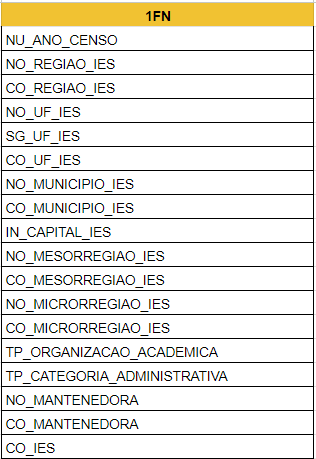
\includegraphics[width=.3\textwidth]{Primeira nominal 1.PNG}
\caption{.}

\centering
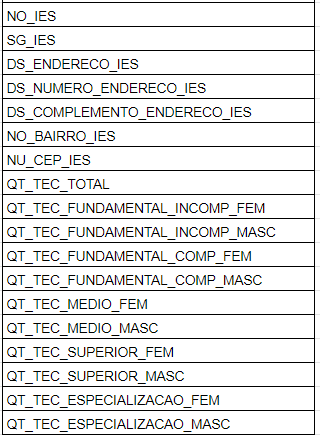
\includegraphics[width=.3\textwidth]{Primeira nominal 2.PNG}
\caption{.}

\centering
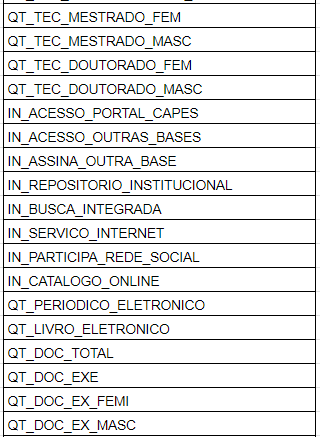
\includegraphics[width=.3\textwidth]{Primeira nominal 3.PNG}
\caption{.}

\centering
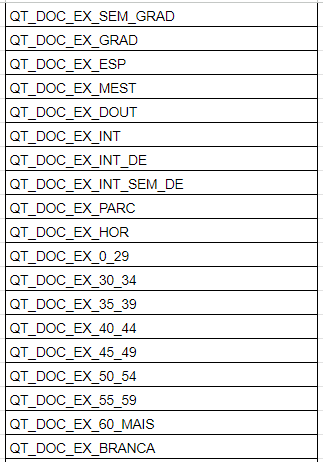
\includegraphics[width=.3\textwidth]{Primeira nominal 5.PNG}
\caption{.}

\centering
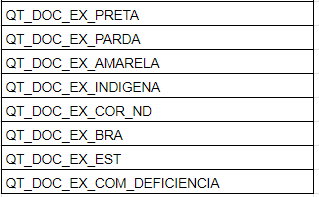
\includegraphics[width=.3\textwidth]{Primeira nominal 6.PNG}
\caption{.}
\end{figure}

A Segunda forma nominal já foi mais detalhada, e teve detalhes também da tabela original.


\begin{figure}[h!]
\centering
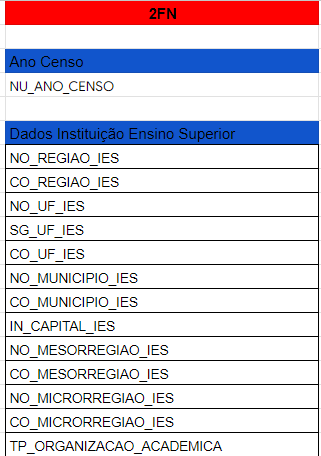
\includegraphics[width=.3\textwidth]{Segunda forma nominal 1.PNG}
\caption{.}

\centering
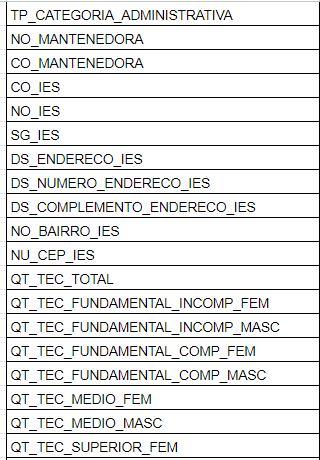
\includegraphics[width=.3\textwidth]{Segunda forma nominal 2.PNG}
\caption{.}

\centering
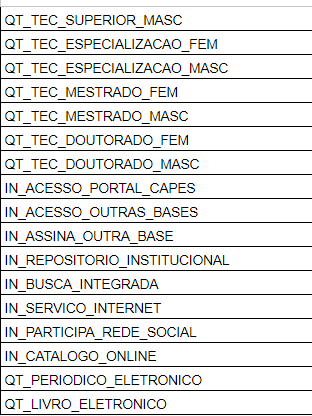
\includegraphics[width=.3\textwidth]{Segunda forma nominal 3.PNG}
\caption{.}

\centering
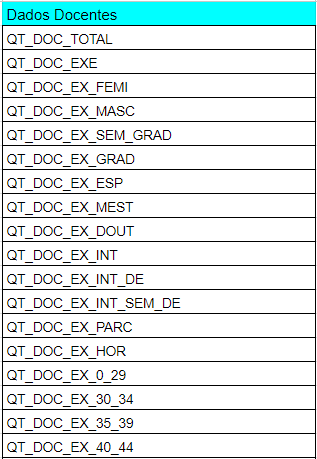
\includegraphics[width=.3\textwidth]{Segunda forma nominal 4.PNG}
\caption{.}

\centering
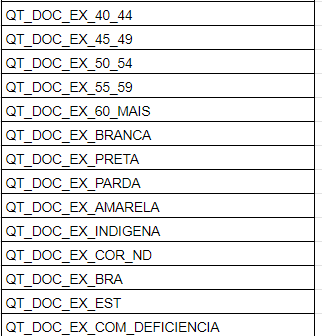
\includegraphics[width=.3\textwidth]{Segunda forma nominal 5.PNG}
\caption{.}

\end{figure}

A terceira forma nominal, agora, bem mais detalhada, e com as partes separando em grande detalhe.

\begin{figure}[h!]
\centering
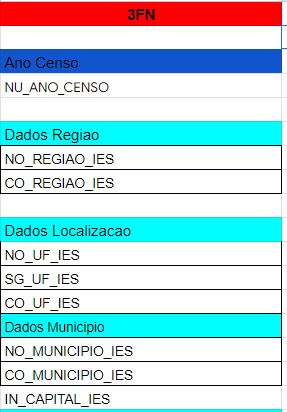
\includegraphics[width=.3\textwidth]{Terceira forma nominal 1.PNG}
\caption{.}

\centering
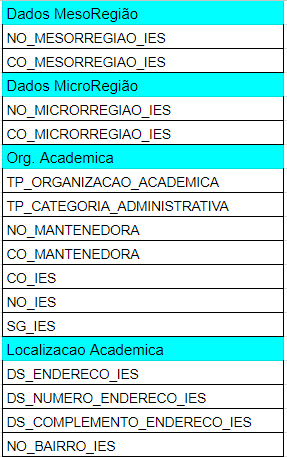
\includegraphics[width=.3\textwidth]{Terceira forma nominal 2.PNG}
\caption{.}

\centering
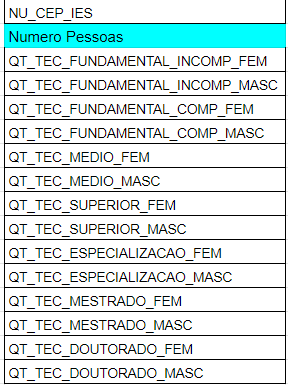
\includegraphics[width=.3\textwidth]{Terceira forma nominal 3.PNG}
\caption{.}

\centering
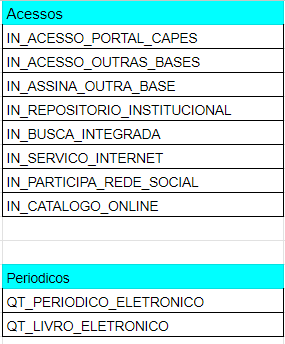
\includegraphics[width=.3\textwidth]{Terceira forma nominal 4.PNG}
\caption{.}

\centering
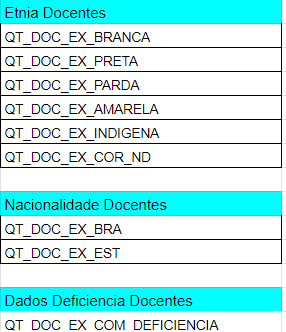
\includegraphics[width=.3\textwidth]{Terceira forma nominal 5.PNG}
\caption{.}

\centering
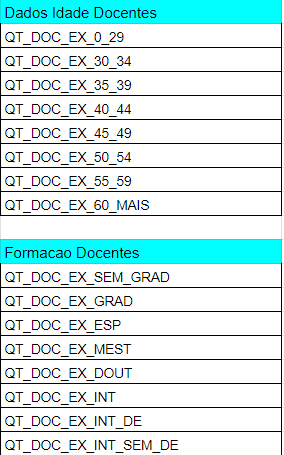
\includegraphics[width=.3\textwidth]{Terceira forma nominal 6.PNG}
\caption{.}

\centering
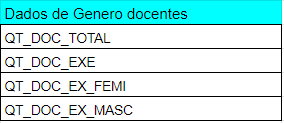
\includegraphics[width=.3\textwidth]{Terceira forma nominal 7.PNG}
\caption{.}

\end{figure}



\section{Projeto Lógico/Relacional}

Seguiu mais a segunda forma nominal, e teve a assistência do professor monitor. O modelo lógico também é bem correlacionado com como a tabela original se portava.

\begin{figure}[h!]
\centering
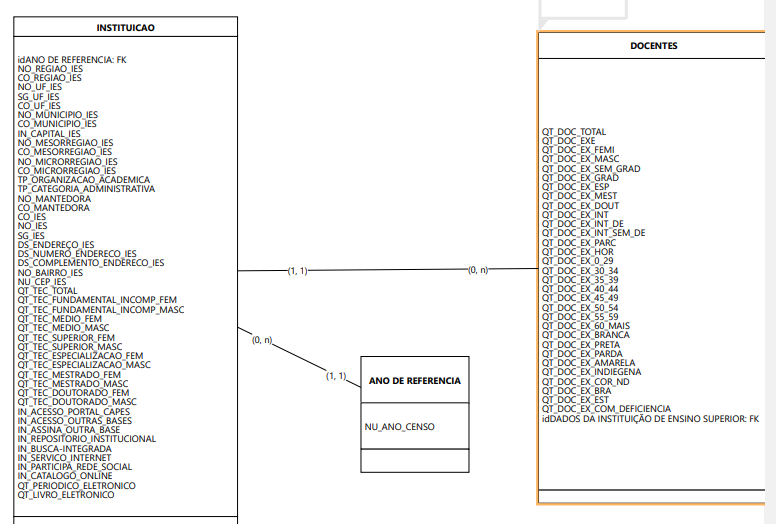
\includegraphics[width=.9\textwidth]{modelo logico.PNG}
\caption{modelo logico}
\end{figure}

\section{Projeto Conceitual}

Esse foi mais baseado na terceira forma nominal. Como pode ser visto, as chaves que mais o definem são relacionadas ao ano (quando há duvidas), pois o censo é baseado em instituições e os dados de cada ano. Por isso o ano tem várias ligações com várias tabelas.

\begin{figure}[h!]
\centering
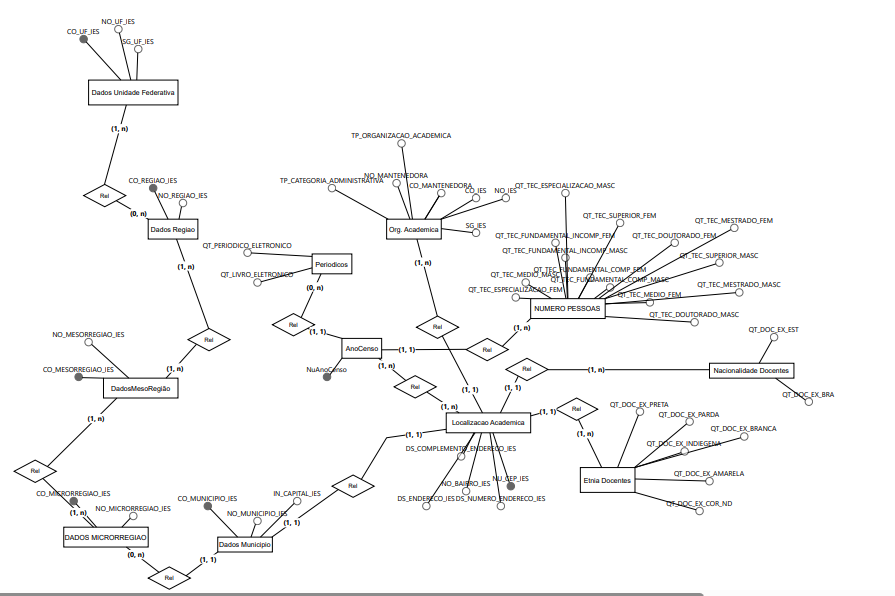
\includegraphics[width=.9\textwidth]{modelo conceitual.PNG}
\caption{modelo relacional}
\end{figure}


\section{Projeto Físico}\label{sec:figs}

Preferi usar o PostgreSQL pra fazer os comandos, e no inicio tava complicado, mas, depois de um tempo, consegui me acostumar com os mecanismos do mesmo 

Algo que me frustrou inicialmente é que achei que fosse necessário fazer um servidor do zero, Descobri rapidamente que esse não era o caso

Usei vários tutoriais que me ajudaram,\cite{videoajuda} e eu tentei sempre usar o Query, pra não só demonstrar entendimento dos conhecimentos aplicados em aula, mas também, porque eu percebi que era mais facil usar o insert, create table, dentre outros comandos.

Aos quais eu também tentei me acostumar, Porque uma coisa é aprender na teoria, e outra diferente é usar a prática.

Mas, felizmente deu tudo certo e o servidor não precisou ser exatamente feito, apenas fiz um novo banco e coloquei uma nova tabela nele, após ver certos tutoriais.

\begin{figure}[h!]
\centering
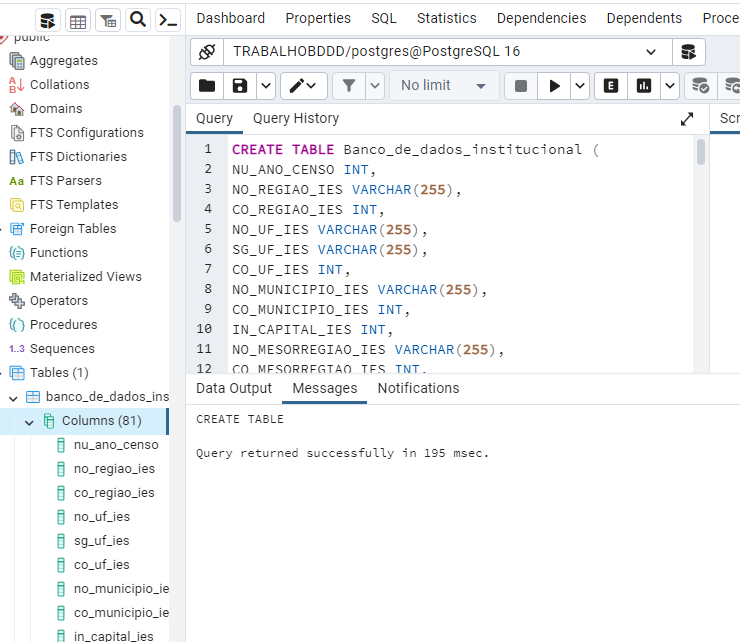
\includegraphics[width=1\textwidth]{tabela criada genuinamente 2.PNG}
\caption{criação da tabela}
\end{figure}

\subsection{Populacao da tabela}
Aqui a tabela está sendo populada pelos dados adequadamente.
\cite{PostgreSQL}
\begin{figure}[h!]
\centering
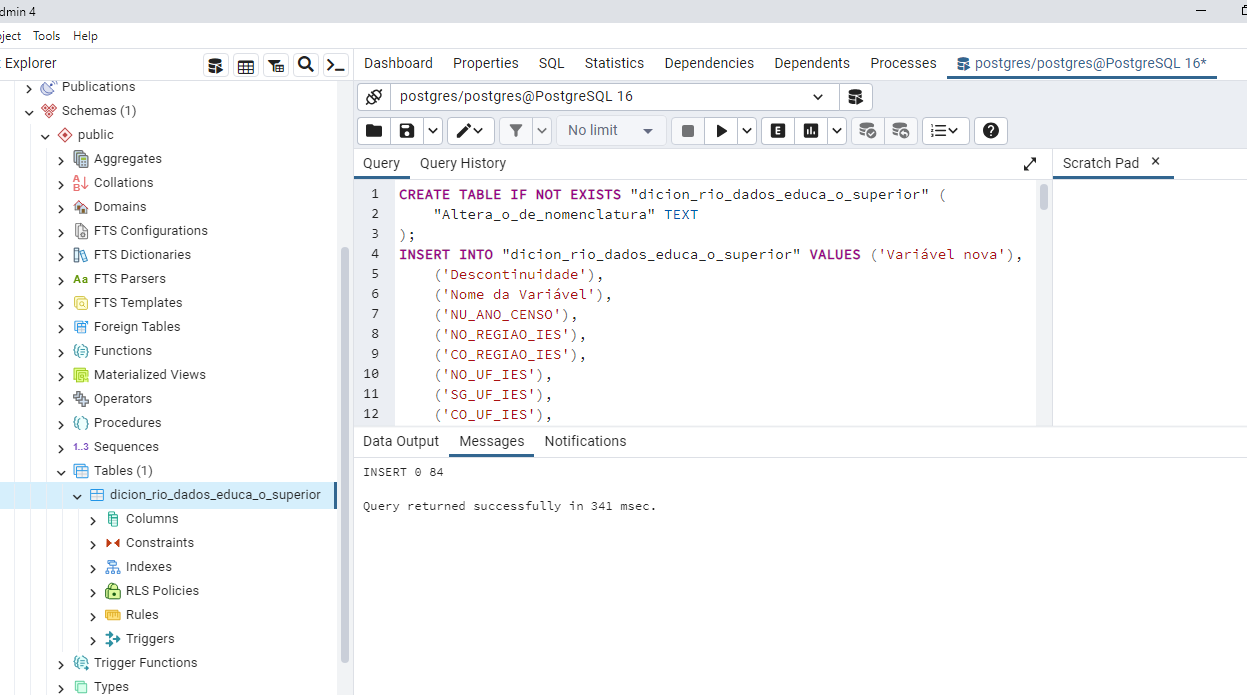
\includegraphics[width=1\textwidth]{tabela criada, dados colocados 1.PNG}
\caption{inserção de dados novos na tabela pra "popular" a mesma.}
\end{figure}

\subsection{Consulta da tabela}
\cite{aulasSQL}
\begin{figure}[h!]
\centering
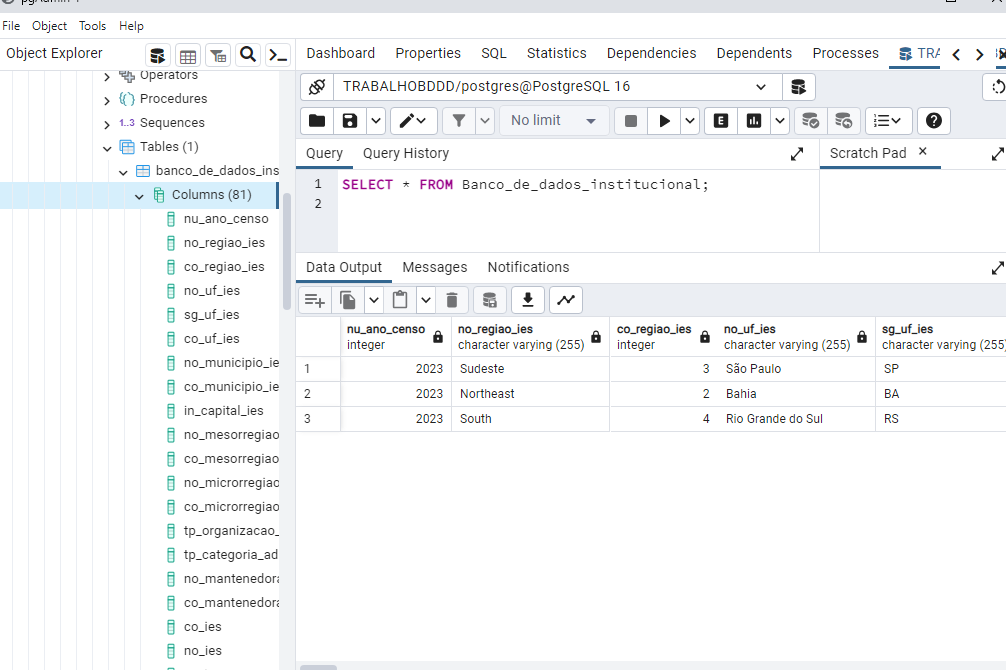
\includegraphics[width=1\textwidth]{consulta da tabela de BDD.PNG}
\caption{consulta da tabela, indicando que os dados realmente entraram.}

\end{figure}


\section{Lições Aprendidas}

Bem, existem projetos e existem projetos. Tivemos que trocar de projeto ao menos 3x em um curto espaço de tempo, e considerando que nós conseguimos realizar o suficiente pra preencher os requisitos, creio que foi de forma adequada. A primeira vez foram por motivos já falados, a segunda foi a inadequação da tabela, e a terceira teve que ter intereferência dos professores para fazer um bom projeto.

Além disso, comecei a melhorar um pouco a familiarização com o SQL, podendo segurá-lo e dominá-lo melhor. Além disso,tivemos que escutar mais os professores durante esse projeto do que de outros. E além disso, a normalização, que era um conceito meio complicado pra nós, agora está mais adequado.

Uma dificuldade que tivemos foi o dominio do Overleaf, com respeito a localização das imagens. Outra questão foi onde conseguir fontes adequadas pra poder melhorar as tabelas, quando na aula não era o suficiente. Não que as aulas tenham sido ruins (elas foram bem boas), mas não tinha o exemplo prático do PostgreSQL, mas era também pra incentivar os alunos a procurarem suas próprias ferramentas.

\section{Referencias}


\bibliographystyle{sbc}
\bibliography{sbc-template}

\end{document}
